%QCM pourcentages / proportions / taux d'évolution / évolutions réciproques

\section{Questions à choix multiple \textit{(6 points)}}\label{ex:qcm}

Cet exercice se présente sous la forme d'un questionnaire à choix multiple (QCM). Les six questions sont indépendantes. Pour chaque question, une seule réponse est exacte, on demande d'indiquer cette réponse sur la copie sans la justifier. Chaque bonne réponse rapporte 1 point, chaque réponse incorrecte retire \num{0.25} point, une question sans réponse n'apporte ni ne retire aucun point. Si le total est négatif, la note est ramenée à 0.
%On inscrira sur sa copie, le numéro de la question et la lettre de la réponse choisie.
\vspace*{0.5cm}

\subsection{En prime}

Le tableau suivant donne le montant en euros et la répartition d'une prime de fin d'année de 250 techniciens et cadres d'un laboratoire d'analyses biologiques. On suppose que dans chaque classe, tous les éléments sont situés au centre.

{\small \begin{center}
	\begin{tabular}{|@{\ }c@{\ }|@{\ }c@{\ }|}
		\hline
		\textbf{Montant de la prime en euros} & \textbf{Effectif} \\ \hline
		[400 ; 500[                         & 25                \\ \hline
		[500 ; 600[                         & 85                \\ \hline
		[600 ; 700 [                        & 75                \\ \hline
		[700 ; 800 [                        & 35                \\ \hline
		[800 ; 900 [                        & 30                \\ \hline
	\end{tabular}
\end{center}}

\begin{questions}
	\question La fréquence de la classe [600 ; 700[ ?
	
	\begin{oneparchoices}
		\choice \num{30};
		\choice \num{0.75};
		\CorrectChoice \num{0.30}.
	\end{oneparchoices} 

	\question La fréquence d'avoir un employé ayant une prime strictement inférieure à 600 € a pour valeur :
	
	\begin{oneparchoices}
		\choice \num{0.34};
		\CorrectChoice \num{0.44};
		\choice \num{0.56}.
	\end{oneparchoices} 

	\question Une valeur approchée arrondie à l'euro de l'écart type est :
	
	\begin{oneparchoices}
		\choice \num{137};
		\choice \num{173};
		\CorrectChoice \num{116}.
	\end{oneparchoices} 
\end{questions}  

\subsection{Avec un digramme statistique}

\begin{multicols}{2}
	Le diagramme suivant donne la répartition en pourcentage des personnels non médecins et des sages-femmes des établissements publics de santé, en 2005.
	Le nombre total de ces personnels était \num{773746}.
	Les infirmiers représentaient \num{40.20} \% des personnels des services de soin. Les aides-soignants représentaient \num{34.38} \% des personnels des services de soin.
	
	
	
	\begin{center}
		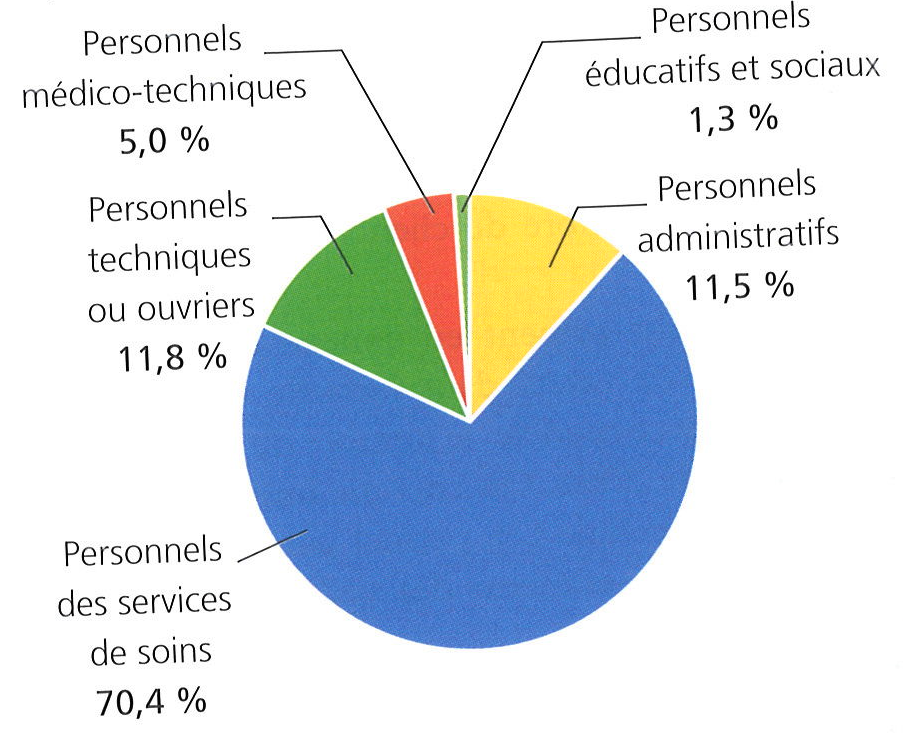
\includegraphics[scale=0.9]{img/repartition}
	\end{center}
	
\end{multicols}


\begin{questions}
	\question La proportion d'infirmiers dans l'ensemble des personnels est environ :
	
	\begin{oneparchoices}
		\choice \num{30.2} \%;
		\CorrectChoice \num{28.3} \%;
		\choice \num{29.6} \%.
		
	\end{oneparchoices} 

	\question Les aides-soignants étaient :
	
	\begin{oneparchoices}
		\choice \num{26586};
		\choice \num{265859};
		\CorrectChoice \num{187274}.
		
	\end{oneparchoices} 

	\question Les personnels éducatifs et sociaux étaient :
	
	\begin{oneparchoices}
		\choice \num{26586};
		\CorrectChoice \num{10059};
		\choice \num{265859}.
		
	\end{oneparchoices} 
\end{questions}